%	The main skeletal structure
	\documentclass[crop,tikz,convert={outext=.svg,command=\unexpanded{pdf2svg \infile\space\outfile}},multi=false]{standalone}%	\documentclass[twocolumn]{report}
	\usepackage{setspace}
	\usepackage{graphicx}
		\DeclareGraphicsExtensions{.pdf,.png,.eps,.svg	ps}
	\usepackage{subcaption}
	\usepackage{lscape}
	\usepackage{pifont}
%	\usepackage{bbding}
	\usepackage{multirow}
	\usepackage{longtable}
	\usepackage[version=4]{mhchem}
	\usepackage{xfrac}
	\usepackage{color}
	\usepackage[colorlinks=true]{hyperref}
	\usepackage{gensymb}
	\usepackage{multicol}
		\setlength{\columnseprule}{0.4pt}
		\setlength{\columnsep}{5mm}
\makeatletter 
\newcounter{reaction} 
%%% >> for article << 
%\renewcommand\thereaction{C\,\arabic{reaction}} 
%%% << for article << 
%%% >> for report and book >> 
\renewcommand\thereaction{C\,\thechapter.\arabic{reaction}} 
\@addtoreset{reaction}{chapter} 
%%% << for report and book << 
\newcommand\reactiontag{\refstepcounter{reaction}\tag{\thereaction}} 
\newcommand\reaction@[2][]{\begin{equation}\ce{#2}% 
\ifx\@empty#1\@empty\else\label{#1}\fi% 
\reactiontag\end{equation}} 
\newcommand\reaction@nonumber[1]{\begin{equation*}\ce{#1}% 
\end{equation*}} 
\newcommand\reaction{\@ifstar{\reaction@nonumber}{\reaction@}} 
\makeatother 


	\usepackage[a4paper]{geometry}
	\usepackage{fullpage}
	\usepackage{fancyhdr}
%		\pagestyle{fancy}
%		\lhead{}
%		\chead{}
%		\rhead{\slshape \rightmark}
%		\fancyhead[LO,RE]{\slshape \leftmark} 
%		\fancyfoot[R]{\thepage} 
%	\renewcommand{\headrulewidth}{0.4pt} 
%	\renewcommand{\footrulewidth}{0.4pt} 
	\usepackage{cite}
	
%	\onehalfspacing
	\renewcommand{\baselinestretch}{1.5}
	
%	Footnote symbols
	\renewcommand{\thefootnote}{\fnsymbol{footnote}}

% Defining the chapter abstract area
%	\newenvironment{abstract}{\rightskip1in}{}

% Allow standard state notation
	\usepackage[varioref=false]{chemstyle}

% Allow for numbered examples
%	\usepackage{theorem,lipsum}
%	\theorembodyfont{\upshape}
%	\newtheorem{example}{Example}[chapter]
%	\newtheorem{question}{Question}[chapter]
%	\newtheorem{exercise}{Exercise}[chapter]
%	\newtheorem{concept}{Key Concept}[chapter]
%%%%%\begin{example}
%%%%%This is an example?
%%%%%\end{example}
%%%%%
%%%%%\begin{question}
%%%%%This is a quesiton?
%%%%%\end{question}

%%%%%FONT STUFF

%\usepackage[defaultfam,extralight,tabular,lining]{montserrat} %% Option 'defaultfam'
%%% only if the base font of the document is to be sans serif
%\usepackage[T1]{fontenc}
%\renewcommand*\oldstylenums[1]{{\fontfamily{Montserrat-TOsF}\selectfont #1}}

\usepackage{arev}
\usepackage[T1]{fontenc}
\usepackage{soul}

%%%%%TIKZ stuff
	\usepackage{tikz}
	\usepackage{pgfplots}
	\usetikzlibrary{decorations.pathmorphing,patterns,arrows,shapes.arrows,shapes}
	\usepgfplotslibrary{fillbetween}
	\tikzset{every picture/.style=remember picture}
		\newcommand{\mathnode}[1]{%
		\mathord{\tikz[baseline=(#1.base), inner sep = 0pt]{\node (#1) {$#1$};}}}

%%%%%% Grey stuff
%Need to define a shitload of greys...
\definecolor{gray1}{RGB}{240,240,240}
\definecolor{gray2}{RGB}{225,225,225}
\definecolor{gray3}{RGB}{210,210,210}
\definecolor{gray4}{RGB}{200,200,200}
\definecolor{gray5}{RGB}{180,180,180}


\begin{document}

\begin{tikzpicture}[scale=1]
  \begin{axis}[
    grid=none,
    axis lines = middle,
%    xmax=10,
    ymax=1.1, 
    ymin = -1.1,
%    axis x line=none,   
   width=10cm,
    height=5cm, 
%    axis y line=none,
%    restrict y to domain=-1:9,
    enlargelimits,
%    xlabel={$x$},
%    xlabel style={ },
%    ylabel={$y$},
%    ylabel style={},
    ticks=none,
%    ylabel near ticks,
%    xlabel near ticks,
    ]
% Incident wave:
	\newcommand \deltaX{0} % Delta wave shift
	\draw[->, thick,black] (axis cs:{(\deltaX+90)/180},1) -- ++ (axis direction cs:0.5,0) node[above]{$v$};
	\draw[->,thick,red] (axis cs:0,{sin(-\deltaX)}) -- ++({atan(2*cos(-\deltaX))}:1cm) node[right]{$F$};
	\draw[densely dotted,red] (axis cs:0,{sin(-\deltaX)}) -- ++(0:0.5cm) node[midway,above]{\footnotesize $\theta$};	\draw[->,ultra thick,cyan] (axis cs:0,{sin(-\deltaX)}) -- ++(axis direction cs:0,{-0.5*cos(\deltaX)}) node[right]{\footnotesize $f$};
	\node[draw,circle,fill=red,inner sep=0pt, minimum size=3pt] at  (axis cs:0,{sin(-\deltaX)}) {};
	\node[] at (axis cs:-0.15,1) {$y$};
	\node[] at (axis cs:4,-0.15) {$x$};

    \addplot[blue,domain=0:3.7,samples=100,] {sin(180*x-\deltaX)}; % Incident pulse
 
\end{axis}

\end{tikzpicture}


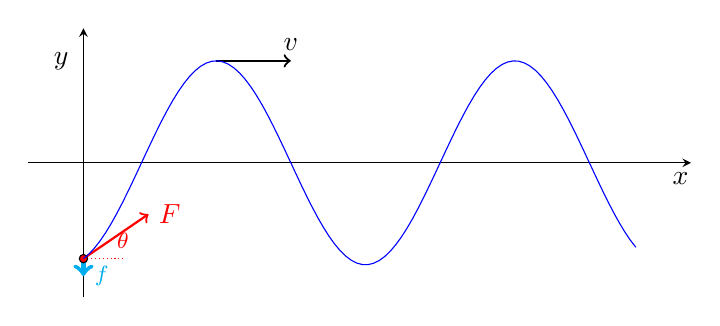
\begin{tikzpicture}[scale=1]
  \begin{axis}[
    grid=none,
    axis lines = middle,
%    xmax=10,
    ymax=1.1, 
    ymin = -1.1,
%    axis x line=none,   
   width=10cm,
    height=5cm, 
%    axis y line=none,
%    restrict y to domain=-1:9,
    enlargelimits,
%    xlabel={$x$},
%    xlabel style={ },
%    ylabel={$y$},
%    ylabel style={},
    ticks=none,
%    ylabel near ticks,
%    xlabel near ticks,
    ]
% Incident wave:
	\newcommand \deltaX{70} % Delta wave shift
	\draw[->, thick,black] (axis cs:{(\deltaX+90)/180},1) -- ++ (axis direction cs:0.5,0) node[above]{$v$};
	
	\draw[->,thick,red] (axis cs:0,{sin(-\deltaX)}) -- ++({atan(2*cos(-\deltaX))}:1cm) node[right]{$F$};
	\draw[densely dotted,red] (axis cs:0,{sin(-\deltaX)}) -- ++(0:0.5cm) node[above]{\footnotesize $\theta$};
	
	\draw[->,ultra thick,cyan] (axis cs:0,{sin(-\deltaX)}) -- ++(axis direction cs:0,{-0.5*cos(\deltaX)}) node[right]{\footnotesize $f$};
	\node[draw,circle,fill=red,inner sep=0pt, minimum size=3pt] at  (axis cs:0,{sin(-\deltaX)}) {};
	\node[] at (axis cs:-0.15,1) {$y$};
	\node[] at (axis cs:4,-0.15) {$x$};

    \addplot[blue,domain=0:3.7,samples=100,] {sin(180*x-\deltaX)}; % Incident pulse
 
\end{axis}

\end{tikzpicture}
\end{document}

% Use the following to include the graphics in the chapter
%
%
%\begin{figure}[htbp]
%\begin{center}
%\includegraphics[scale=1]{ch-x/images/filename.pdf}
%\caption[Caption for list of figures]{Full caption to appear beside the image}
%\label{fig:label}
%\end{center}
%\end{figure}
 